%\cite{verb2014} Multivariate mixture of Erlangs same data

%\cite{Alai2013} lifetime data for different cohorts of the Norwegian population and annuity valuation for truncated lifetimes using
%truncated multivariate Gamma distribution

%\cite{Lee2012} apply truncated multivariate Gaussian mixture models for truncated flow cytometry data.


  \begin{figure}
  \centering
    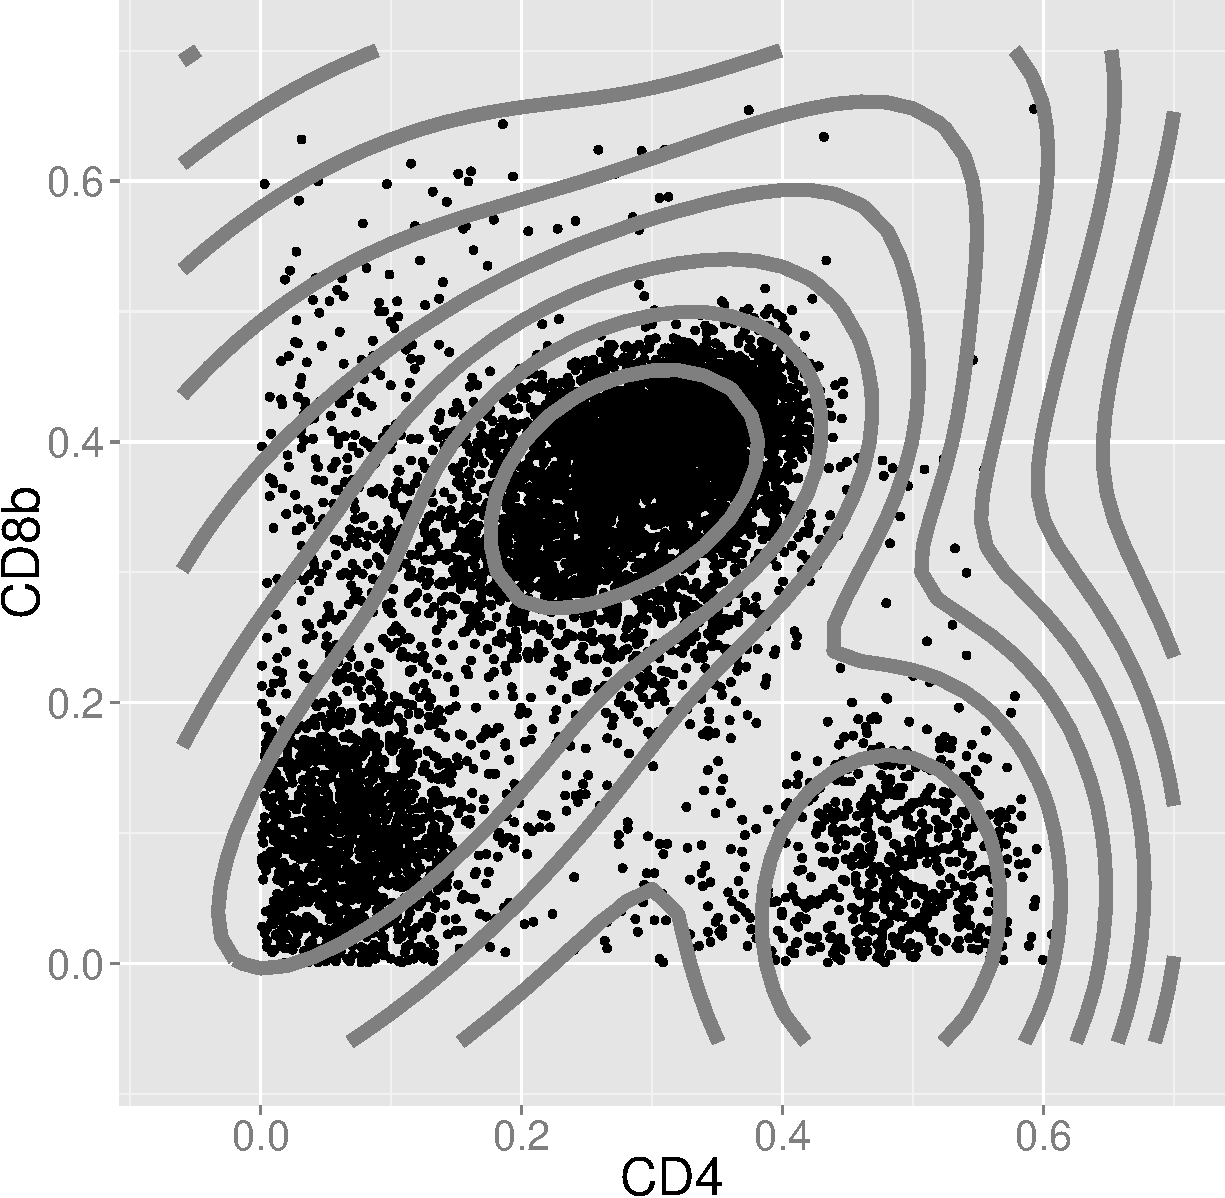
\includegraphics[width=.27\textwidth]{figs/gvhd_control.pdf}
    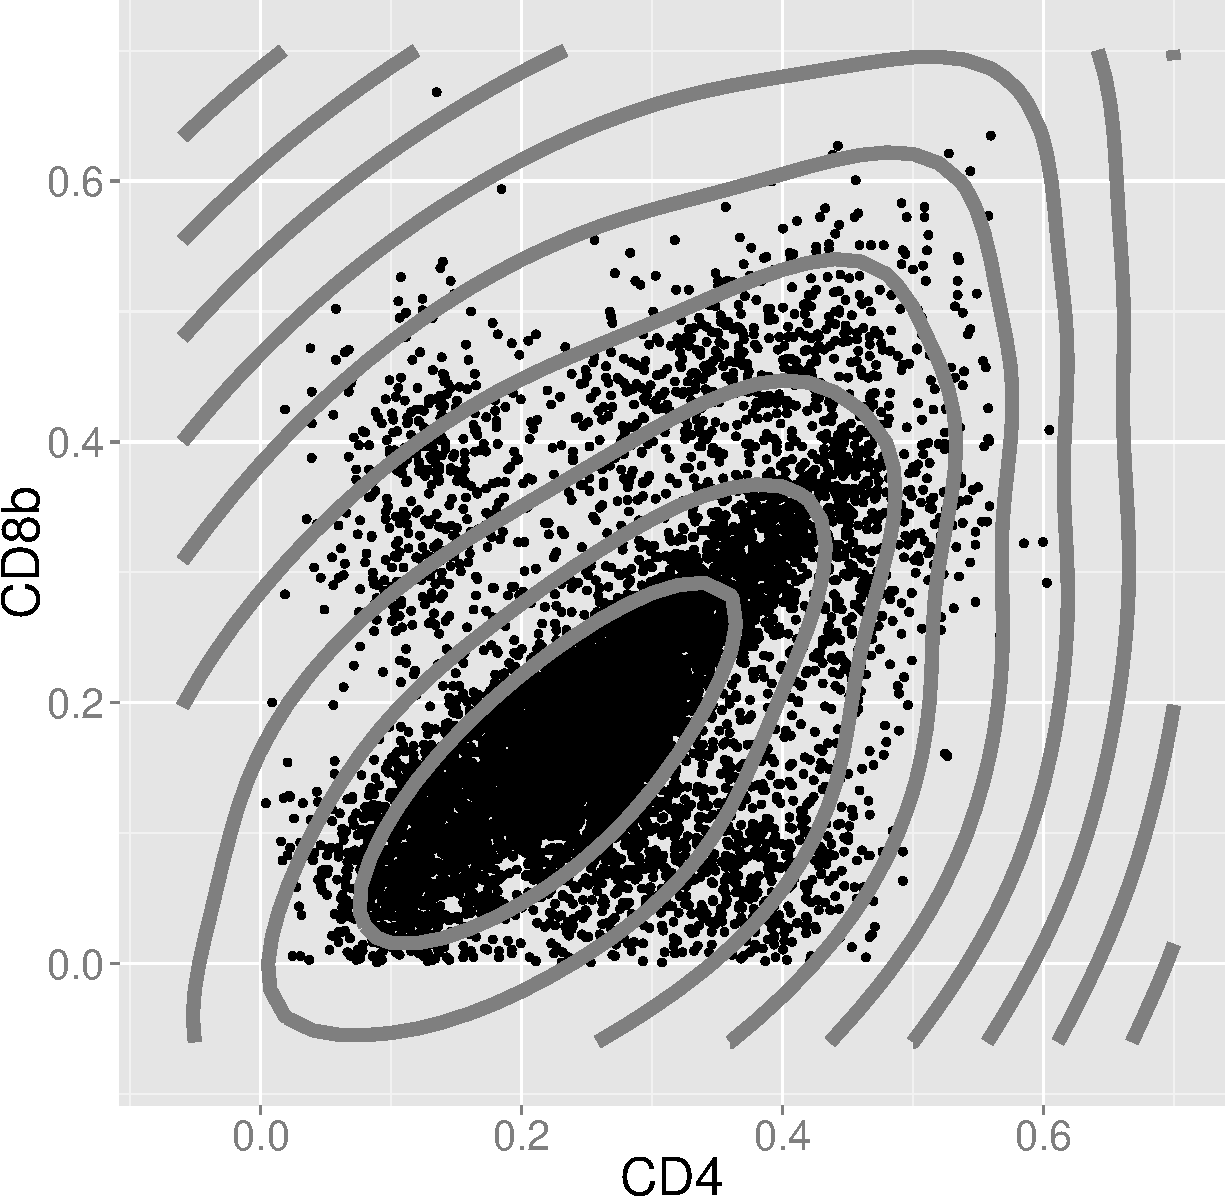
\includegraphics[width=.27\textwidth]{figs/gvhd_pos.pdf}
\caption{ Scatterplots of first two dimensions for control (left) and positive (right) group. Contours represent
log posterior-mean densities under a Dirichlet process mixture.}
  \label{fig:plot_gvhd}
  \end{figure}

We apply our algorithm to a dataset of flow cytometry measurements from patients subjected to bone-marrow transplant~\citep{Brink07}. This graft-versus-host disease
dataset has 6,809 control and 9,083 positive observations, corresponding to whether donor immune cells attack host cells.
Each observation consists of four biomarker measurements truncated between 0 and 1,024, though more complicated truncation rules are often 
used according to operator judgement~\citep{Lee2012}. We normalize and plot the first two dimensions, markers CD4 and CD8b, in 
Figure \ref{fig:plot_gvhd}.
Truncation complicates the clustering of observations into homogeneous groups, an important step in the flow-cytometry pipeline called
gating.
Consequently,~\cite{Lee2012} propose an expectation-maximization algorithm for truncated Gaussian mixture models, which must be adapted if
different mixture components or truncation rules are used. 

%We regard the normalized observations as the output of a rejection sampling algorithm that discards proposals outside the unit hypercube.
%After imputing these according to algorithm \ref{alg:rej_sim}, we can easily apply standard Bayesian models without worrying about 
%edge effects and missing probability.
We model the untruncated distribution for each group as a Dirichlet process mixture of Gaussian kernels~\citep{Lo1984}, with points
outside the four-dimensional unit hypercube discarded to form the normalized dataset.
The Dirichlet process mixture model is a flexible nonparametric prior over densities %that bypasses model selection issues like
%choosing the number of components in a Gaussian mixture model, and is 
parametrized by a concentration parameter $\alpha$ and a base probability measure.
We set $\alpha = 1$, and for the base measure, which gives the distribution over cluster parameters, we use a normal-inverse-Wishart distribution. 
%There exist standard techniques to both sample new data points for a Dirichlet process mixture, as well as to sample parameters given the augmented 
%data.
Given the rejected variables, we can use standard techniques to update a representation of the Dirichlet process. 
We follow the blocked-sampler of~\cite{IshJam2001} based on the stick-breaking representation of the Dirichlet process, using a truncation level of 
50 clusters. 
This corresponds to updating $\theta$, step 2 in Algorithm~\ref{alg:rej_post}. 
Having done this, we discard the old rejected samples, and produce a new set by drawing from a 50-component Gaussian mixture 
model, corresponding to step 1 in Algorithm~\ref{alg:rej_post}.

Figure~\ref{fig:plot_gvhd} shows the log mean posterior densities for the first two dimensions from 10,000 iterations. %Control vs Pos.
While the control group has three clear modes, these are much less pronounced in the positive group.
Directly modeling observations with a Gaussian mixture model obscured this by forcing modes away from the edges. 
One can use components with bounded support in the mixture model, such as a Dirichlet process mixture of Beta densities; however, these do not reflect the 
underlying data generation process, and are unsuitable when different groups have different
truncation levels. By contrast, it is easy to extend our modeling ideas to allow groups to share
%components \citep{TehJorBea2006}, thereby allowing better identification of disease predictors.
components, allowing better identification of disease predictors.

Our sampler took less than two minutes to run 1,000 iterations, not much longer than a typical Dirichlet process sampler for 
datasets of this size. The average number of augmented points was 3,960 and 4,608 for the two groups. We study our  sampler more systematically 
in the next section, but this application demonstrates the flexibility and simplicity of our main idea.

%this can easily be extended to identify shared clusters among the two groups \cite{Teh2006}.


